\section{Experimental Setup}
We evaluated the performance of OHA* and A* on a set of 120 octile-based maps, ranging in size from 50x50 
to 320x320, which we borrowed from BioWare's popular role-playing game \emph{Baldur's Gate 2}. 
This is a commonly used benchmark that frequently appears in pathfinding research 
\cite{botea04,bjornsson05,bjornsson06,sturtevant05,harabor08}.
We believe it is sufficiently representative of scenarios typical to modern video games. 
\begin{figure}[t]
       \begin{center}
                       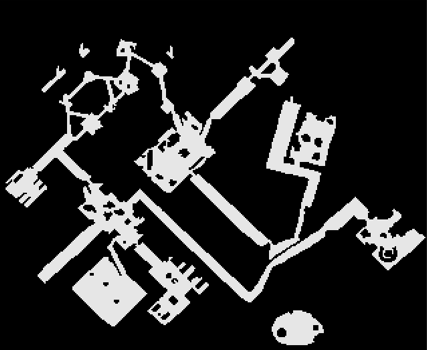
\includegraphics[scale=0.50, trim = 10mm 10mm 10mm 0mm]{diagrams/bgmap.png}
       \end{center}
	\vspace{-3pt}
       \caption{An example map from BioWare's \emph{Baldur's Gate 2}}
       \label{fig-bgmap}
\end{figure}
In addition we also evaluate six variants of the demo map from Figure \ref{fig-oha_contrast},
 which is distributed with the University of Alberta's freely available pathfinding library 
Hierarchical Open Graph\footnote{\url{www.cs.ualberta.ca/~nathanst/hog.html}} (or HOG).
We designate these variants \emph{R0, R10, R20, R30, R40, R50}.
In each case the numeric constant refers to the probability that each traversable tile 
in the original map will be be flipped to become an obstacle.
We perform this evaluation in order to measure OHA*'s worst-case performance which we expect will occur in 
environments that are densely packed with obstacles.
\par
For each map we generated 100 experiments by randomly creating valid problems between arbitrarily chosen 
pairs of start and goal locations.
Each algorithm solved every problem once making for a total of 25200 (126 $\times$ 200) distinct experiments.
All experiments were conducted on a 1.83GHz Intel Core 2 Duo processor with 1GB RAM running OSX 10.5.4.
Both A* and OHA* were implemented using HOG. 
